\subsection{Documentazione}
    \subsubsection{Descrizione}
      Questa sezione fornisce le norme per la stesura, la verifica e l'approvazione dei documenti. Tali regole vanno seguite in tutti i documenti ufficiali prodotti durante il ciclo di vita del software, garantendo così la coerenza e la validità degli stessi.

    \subsubsection{Ciclo di vita dei documenti}
      Ogni documento attraversa diversi stadi:
      \begin{itemize}
        \item \textbf{Creazione e strutturazione del documento:} il documento viene creato nella sua directory di appartenenza (secondo le indicazioni presenti nella sezione "Documenti interni ed esterni"), e viene stesa la sua struttura generale. Viene utilizzato un template\ped{\textit{G}} \LaTeX{}\ped{\textit{G}} (descritto nella sezione \textsection3.1.5.1);
        \item \textbf{Stesura:} scrittura effettiva dei contenuti del documento da parte di un redattore\ped{\textit{G}};
        \item \textbf{Verifica:} attività eseguita dai Verificatori, i quali si occupano di controllare che il documento sia conforme alle \textit{\NdP{} 2.0.0}, sia sintatticamente che semanticamente. Alla fine di ogni controllo, il resoconto della verifica viene consegnato al Responsabile di Progetto che provvede a notificare il redattore\ped{\textit{G}} in caso di errori, riportando il documento al passo di "Stesura". Quando la fase di verifica finale non rileva ulteriori errori, il Responsabile passa il documento al processo di "Approvazione";
        \item \textbf{Approvazione:} in questa fase i Verificatori hanno terminato i controlli finali con esito positivo, comunicandoli al Responsabile, il quale si occupa di approvare il documento e preparare il rilascio.
      \end{itemize}

    \subsubsection{Documenti interni ed esterni}
      Ogni documento deve essere classificato come Interno o Esterno:
      \begin{itemize}
        \item \textbf{Interno:} il documento viene utilizzato all'interno del team;
        \item \textbf{Esterno:} il documento viene condiviso con il Committente\ped{\textit{G}} ed il Proponente\ped{\textit{G}}.
      \end{itemize}

    \subsubsection{Documenti presenti}
      Di seguito sono elencati i documenti ufficiali che verranno prodotti e la loro classificazione in uso Interno o Esterno.
      \subsubsubsection{Norme di Progetto}
        Documento ad uso Interno.\\
        Lo scopo delle \textit{\NdP{}} è descritto nella sezione \textsection1.1 "Scopo del Documento", di questo stesso documento.\\

      \subsubsubsection{Studio di Fattibilità}
        Documento ad uso Interno.\\
        Lo \textit{\SdF{}} ha l'obiettivo di esporre (brevemente) ogni capitolato\ped{\emph{G}} e di elencare per ognuno gli aspetti positivi e le criticità che il team ha individuato.

      \subsubsubsection{Glossario}
        Documento ad uso Esterno.\\
       	Il \Glossario{}  ha lo scopo di disambiguare alcuni termini che compaiono all'interno dei documenti e vengono utilizzati nelle comunicazioni interne.

      \subsubsubsection{Analisi dei Requisiti}
        Documento ad uso Esterno.\\
        Lo  scopo  dell'\textit{\AdR{}} è di esporre dettagliatamente i requisiti individuati per lo sviluppo del capitolato\ped{\emph{G}} scelto.

      \subsubsubsection{Piano di Progetto}
        Documento ad uso Esterno.\\
        Lo scopo del \textit{\PdP{}} è di organizzare le attività in modo da gestire le risorse disponibili in termini di tempo e "forza lavoro".

      \subsubsubsection{Piano di Qualifica}
        Documento ad uso Esterno.\\
        Lo scopo del \textit{\PdQ{}} è di presentare i metodi di verifica e validazione implementati dal gruppo, per garantire la qualità del prodotto\ped{\textit{G}} e dei processi adottati.

    \subsubsection{Struttura dei documenti}
      \subsubsubsection{Template \LaTeX}
        Per uniformare la struttura dei documenti il gruppo ha deciso di creare un template\ped{\textit{G}} \LaTeX{}\ped{\textit{G}}, da utilizzare per la stesura di tutti i documenti ufficiali. Il template\ped{\textit{G}} è contenuto nella cartella \LaTeX{}\ped{\textit{G}}, la cui struttura è la seguente:
        \begin{itemize}
          \item \textbf{common\_commands.tex:} file che contiene la definizione di nuovi comandi \LaTeX{}\ped{\textit{G}} per l'inserimento nel flusso di testo di termini ricorrenti:
            \begin{itemize}
              \item \textbf{informazioni sul gruppo:} nome del gruppo e indirizzo email;
              \item \textbf{informazioni sul progetto:} nome del progetto e nomi del Proponente\ped{\textit{G}} e del Committente\ped{\textit{G}};
              \item \textbf{membri del gruppo:} nomi dei membri del gruppo \Gruppo;
              \item \textbf{nomi dei documenti:} nomi dei documenti ufficiali.
            \end{itemize}
          \item \textbf{configs.tex:} contiene i comandi per l'inclusione dei necessari pacchetti \LaTeX{}\ped{\textit{G}} e la definizione dell'aspetto grafico generale dei documenti;
          \item \textbf{copertina.tex:} contiene il codice \LaTeX{}\ped{\textit{G}} per la copertina, ovvero la prima pagina di ogni documento (la cui struttura è descritta nella sezione \textsection3.1.5.2);
          \item \textbf{Template:} directory che contiene la struttura "classica" di un documento (quest'ultima viene descritta di seguito).
        \end{itemize}
        La directory Template ha la seguente struttura:
        \begin{itemize}
          \item \textbf{config:} directory che contiene un solo file: "commands.tex", all'interno del quale sono inseriti dei comandi specifici per il documento considerato (es. nome del documento, stato di approvazione, ecc...). I comandi devono essere adeguatamente modificati per ogni rispettivo documento;
          \item \textbf{res:} directory che contiene due cartelle:
            \begin{itemize}
              \item \textbf{img:} contiene le immagini utilizzate all'interno del documento;
              \item \textbf{sections:} contiene le varie sezioni del documento e un file "changelog.tex", ovvero il codice per il registro delle modifiche.
            \end{itemize}
          \item \textbf{document.tex:} il file contiene la struttura generica di un documento, includendo le sezioni necessarie contenute nella cartella res.
        \end{itemize}
        %da espandere

      \subsubsubsection{Copertina}
        La copertina è la prima pagina di ogni documento e contiene alcune informazioni generali:
        \begin{itemize}
          \item Logo del gruppo \Gruppo{};
          \item Nome del gruppo e nome del capitolato\ped{\emph{G}} scelto: \Gruppo{} - \NomeProgetto{};
          \item Nome del documento (nel caso dei Verbali\ped{\textit{G}} accompagnato dalla data della riunione).
        \end{itemize}
        Queste informazioni sono seguite da una struttura tabellare, che contiene dettagli pertinenti al singolo documento:
        \begin{itemize}
          \item \textbf{Versione:} versione attuale del documento (vedi sezione \textsection3.2);%aggiungere sezione norme di Versionamento
          \item \textbf{Approvazione:} nome e cognome del Responsabile di progetto;
          \item \textbf{Redazione:} nome e cognome dei redattori\ped{\textit{G}} del documento;
          \item \textbf{Verifica:} nome e cognome dei Verificatori;
          \item \textbf{Stato:} stato del ciclo di vita in cui si trova il documento (vedi sezione \textsection3.1.4.1 paragrafo "Ciclo di vita dei documenti");
          \item \textbf{Uso:} indica se il documento è ad uso Interno o Esterno;
          \item \textbf{Destinato a:} elenco dei destinatari del documento (vedi sezione \textsection3.1.4.1 paragrafo del singolo documento);
    	\end{itemize}
    	Tale struttura è infine seguita da alcune informazioni aggiuntive, allineate al centro del documento:
    	\begin{itemize}
          \item \textbf{Descrizione:} breve descrizione del documento;
          \item \textbf{Email:} indirizzo email del gruppo \Gruppo{}.
   		\end{itemize}

      \subsubsubsection{Registro delle modifiche}
        Inizia nella seconda pagina del documento e contiene un resoconto delle modifiche apportate al documento, strutturate in forma tabellare.\\
        Questa sezione è presente anche nei Verbali\ped{\textit{G}} di riunione, nei quali si limita alla stesura, la verifica e l'approvazione del documento in questo ordine, per evitare modifiche retroattive ai Verbali.\\
        Ogni riga rappresenta una modifica ed è suddivisa in cinque colonne:
        \begin{itemize}
          \item \textbf{Versione:} aggiornamento progressivo della versione; 
          \item \textbf{Data:} data della modifica;
          \item \textbf{Nominativo:} nome e cognome del membro del gruppo che ha effettuato la modifica;
          \item \textbf{Ruolo:} ruolo ricoperto in quel momento dal membro del team che ha effettuato la modifica;
          \item \textbf{Descrizione:} breve descrizione della modifica effettuata.
        \end{itemize}

      \subsubsubsection{Indice}
        L'indice si trova nella pagina successiva e ha lo scopo di aiutare nella navigazione del documento e riassumerne la struttura in maniera visuale.\\
        Nell'indice sono elencati i numeri delle sezioni, seguiti dal titolo e dal numero di pagina. Ogni riga dell'indice è un link che porta alla sezione specificata del documento.\\
        L'indice dei contenuti puó essere seguito da un indice delle immagini e un indice delle tabelle.

      \subsubsubsection{Contenuto}
        Tutte le pagine successive sono occupate dal contenuto e sono strutturate come segue:
        \begin{itemize}
          \item in alto a destra il nome del documento;
          \item in alto a sinistra il logo del gruppo \Gruppo{};
          \item il contenuto della pagina diviso da intestazione e piè di pagina con una riga orizzontale;
          \item in basso a destra il numero di pagina nel formato:
          \begin{center}
            \textbf{Pagina [numero di pagina] di [numero totale di pagine]}.
          \end{center}
        \end{itemize}

      \subsubsubsection{Verbali}
        Seguono la stessa struttura generale degli altri documenti, ma hanno un'organizzazione specifica del contenuto, in particolare sono suddivisi in:
        \begin{itemize}
          \item \textbf{Informazioni generali:} che contengono le informazioni dell'incontro e l'ordine del giorno.

             Le informazioni dell'incontro sono:
               \begin{itemize}
                 \item \textbf{Luogo:} il luogo dove si è svolta la riunione (in alternativa il mezzo utilizzato es. Skype\ped{\textit{G}});
                 \item \textbf{Data:} il giorno in cui si è svolta la riunione;
                 \item \textbf{Ora di inizio:} l'orario di inizio della riunione;
                 \item \textbf{Ora di fine:} l'orario di fine della riunione;
                 \item \textbf{Partecipanti:} elenco dei partecipanti alla riunione;
                 \item \textbf{Segretario:} redattore\ped{\textit{G}} del \Verbale{}\ped{\textit{G}}.
               \end{itemize}
			L'ordine del giorno contiene un elenco degli argomenti di discussione previsti per l'incontro.
          \item \textbf{\Verbale{}}\ped{\textit{G}}\textbf{:} che contiene la descrizione e un riassunto degli argomenti elencati nell'ordine del giorno, suddivisi in sezioni;
          \item \textbf{Riepilogo delle decisioni:} contiene il resoconto delle decisioni prese durante la riunione, in forma tabellare. Ogni decisione è identificata da un codice scritto in forma:
          \begin{center}
            \textbf{V[T]\_[numero dell'incontro].[numero progressivo]}
          \end{center}
          dove [T] indica il tipo di \Verbale{}\ped{\textit{G}} che puó essere Interno (I) o Esterno (E).
        \end{itemize}

    \subsubsection{Norme tipografiche}
      \subsubsubsection{Nomi dei file}
        I nomi dei file seguono le seguenti regole:
        \begin{itemize}
          \item sono composti di diverse parole, con la prima lettera minuscola, fatta eccezione per i Verbali che, come descritto in seguito, iniziano per VI oppure VE;
          \item ogni parola è separata da un underscore;
          \item il nome del file corrisponde al nome del documento senza escludere le preposizioni, ad eccezione dei Verbali\ped{\textit{G}}, come già menzionato.
        \end{itemize}
        I Verbali seguono quindi delle regole differenti, a causa della loro unicità rispetto ad altri documenti. Sono nominati seguendo la struttura:
        \begin{center}
          \textbf{{V[T]\_[data]}}
        \end{center}
        \begin{itemize}
          \item \textbf{[T]:} indica il tipo di \Verbale{}\ped{\textit{G}} che puó essere Interno (I) o Esterno (E);
          \item \textbf{[data]:} indica la data della riunione in formato "YYYY\_MM\_DD", ovvero anno (YYYY), mese (MM) e giorno (DD), separati da underscore.
        \end{itemize}
        Esempi di nomi corretti:
        \begin{itemize}
          \item per un documento qualunque: nome\_di\_file.tex;
          \item per un \Verbale{}\ped{\textit{G}}: VI\_2020\_03\_16.tex.
        \end{itemize}
    	\noindent Inoltre, si è deciso di adottare delle convenzioni anche per la parola "verbale", in particolare: 
    	\begin{itemize}
    		\item nel caso in cui essa compaia al singolare, deve essere riportata in corsivo e con la prima lettera maiuscola; 
    		\item nel casi in cui essa compaia al plurale, deve essere riportata solamente con la prima lettera maiuscola. 
    	\end{itemize}

      \subsubsubsection{Stile del testo}
        Le seguenti norme vanno seguite per l'utilizzo di particolari stili di testo:
        \begin{itemize}
          \item \textbf{Grassetto:} usato se necessario all'inizio delle voci di un elenco puntato, a titoli o a termini significativi;
          \item \textbf{Corsivo:} usato per evidenziare proposizioni particolari all'interno del testo, in particolare il nome dei documenti ufficiali, il nome del Proponente\ped{\textit{G}}, il nome del progetto \textit{\NomeProgetto} e il nome del gruppo \textit{\Gruppo{}};
          \item \textbf{Maiuscoletto:} usato per la "G" a pedice che indica le parole presenti nel \Glossario{}.
        \end{itemize}
        Quando all'interno del testo vengono riferiti dei particolari documenti (es.: \AdR), vanno seguite le seguenti regole:
        \begin{itemize}
          \item indicare con lettera maiuscola le iniziali (es. \AdR), senza la versione del documento, il tutto in corsivo;
          \item se si fa riferimento al documento vero e proprio o a qualcosa in esso contenuto, va aggiunta la versione del documento nel formato:
          \begin{center}
              \textbf{v[X].[Y].[Z]}
          \end{center}
          (es. Riferendosi ad una sezione specifica "[\dots{}] come indicato nella \textsection5.1 dell'\AdR{} v1.1.0[\dots{}]").
        \end{itemize}
      \subsubsubsection{Termini del Glossario}
      	Le norme relative ai termini da inserire nel \Glossario{} sono:
        \begin{itemize}
          \item ogni termine del \Glossario{} deve essere contrassegnato, in ogni sua istanza, da una G maiuscola a pedice;
          \item le istanze dei termini del \Glossario{} presenti nei titoli non necessitano della G maiuscola a pedice.
        \end{itemize}

      \subsubsubsection{Elenchi puntati}
          Ogni voce di un elenco puntato deve aderire alle norme seguenti:
          \begin{itemize}
            \item deve iniziare con la lettera minuscola;
            \item deve essere seguita da un ";", fatta eccezione per l'ultimo elemento che deve essere seguito da un punto;
            \item puó iniziare con dei termini in grassetto e/o con prima lettera maiuscola nel caso in cui il resto della voce sia una descrizione di quei termini.
          \end{itemize}

      \subsubsubsection{Date e orari}
        In conformità allo standard ISO 8601, le date devono essere scritte usando il formato:
        \begin{center}
          \textbf{YYYY-MM-DD}
        \end{center}
        ovvero anno in quattro cifre (YYYY), mese in due cifre (MM) e giorno in due cifre (DD).\\
        Gli orari devono essere scritti usando il formato:
        \begin{center}
          \textbf{HH.MM}
        \end{center}
        ovvero l'ora in due cifre (HH) e i minuti in due cifre (MM).

      \subsubsubsection{Tabelle e immagini}
        Le tabelle sono sempre corredate da un titolo ed un'indicizzazione separata dal normale contenuto.\\
        Le immagini sono accompagnate da una didascalia ed un'indicizzazione, anch'essa separata dal normale contenuto.

      \subsubsubsection{Sigle e abbreviazioni}
        Nella stesura dei documenti possono venire menzionate diverse sigle:
        \begin{itemize}
          \item sigle per i ruoli di progetto:
            \begin{itemize}
              \item \textbf{Rp:} Responsabile di Progetto;
              \item \textbf{As:} Amministratore;
              \item \textbf{An:} Analista;
              \item \textbf{Pt:} Progettista;
              \item \textbf{Pr:} Programmatore;
              \item \textbf{Vf:} Verificatore.
            \end{itemize}
          \item sigle per i nomi dei documenti:
            \begin{itemize}
              \item \textbf{SdF:} Studio di Fattibilità;
              \item \textbf{PdQ:} Piano di Qualifica;
              \item \textbf{PdP:} Piano di Progetto;
              \item \textbf{NdP:} Norme di Progetto;
              \item \textbf{AdR:} Analisi dei Requisiti;
              \item \textbf{G:} Glossario.
            \end{itemize}
          \item sigle per revisioni del progetto:
            \begin{itemize}
              \item \textbf{RR:} Revisione dei Requisiti;
              \item \textbf{RP:} Revisione di Progettazione;
              \item \textbf{RQ:} Revisione di Qualifica;
              \item \textbf{RA:} Revisione di Accettazione.
            \end{itemize}
        \end{itemize}

	\subsubsection{Metriche}
		\subsubsubsection{Indice di Gulpease}
			\begin{itemize}
				\item{\textbf{Descrizione}}: è un indice di leggibilità di un testo tarato sulla lingua italiana. Considera due variabili linguistiche: la lunghezza della parola e la lunghezza della frase rispetto al numero di lettere;
				\item{\textbf{unità di misura}}: la metrica è espressa tramite un numero intero;
				\item{\textbf{formula}}: $ IG=89+\frac{300 \times \#frasi -10\times \#lettere}{\#parole} $;
				\item{\textbf{risultato}}: il risultato è compreso tra 0 e 100, dove il valore 100 indica il grado più alto di leggibilità e 0 il più basso. In particolare:
					\begin{itemize}
						\item se il risultato è inferiore a 80, il testo è considerato di difficile lettura per chi ha la licenza elementare; 
						\item se il risultato è inferiore a 60, il documento è considerato di difficile lettura per chi ha la licenza media; 
						\item se il risultato è minore di 40, il documento è considerato di difficile lettura per chi ha un diploma superiore. 
					\end{itemize}
			\end{itemize}
	
		\subsubsubsection{Formula di Flesch}
		\begin{itemize}
			\item{\textbf{Descrizione}}: formula utilizzata per misurare la leggibilità di un testo inglese;
			\item{\textbf{unità di misura}}: la metrica è espressa tramite un numero decimale;
			\item{\textbf{formula}}: $ F = 206,835 - (84,6 \times S) - (1,015 \times P) $, dove: 
				\begin{itemize}
					\item S indica il numero medio di sillabe per parola; 
					\item P indica il numero medio di parole per frase. 
				\end{itemize}
			\item{\textbf{risultato}}: il risultato è compreso tra 0.0 e 100.0, in particolare: 
				\begin{itemize}
					\item se il risultato è compreso tra 0.0 e 30.0 il documento è considerato molto difficile da leggere, adatto a lettori laureati; 
					\item se il risultato è compreso tra 30.0 e 50.0 il documento è leggibile per studenti universitari; 
					\item se il risultato è compreso tra 50.0 e 70.0 il documento è leggibile per chi possiede un diploma superiore; 
					\item se il risultato è compreso tra 70.0 e 90.0 il documento è leggibile per chi possiede una licenza media; 
					\item se il risultato è compreso tra 90.0 e 100.0 il documento viene considerato di facile lettura per un qualsiasi lettore.
				\end{itemize}
		\end{itemize}
	
		\subsubsubsection{Correttezza ortografica}
		\begin{itemize}
			\item{\textbf{Descrizione}}: permette di misurare la correttezza a livello lessicografico del documento;
			\item{\textbf{unità di misura}}: la metrica è espressa tramite un numero intero;
			\item{\textbf{formula}}: il valore coincide con il numero di errori ortografici presenti, cioè: $ CO = \#numero\_errori\_ortografici $;
			\item{\textbf{risultato}}: 
				\begin{itemize}
					\item se il risultato è pari a 0, il documento è considerato corretto e non presenta errori ortografici; 
					\item se il risultato è maggiore di 0, allora il documento presenta almeno un errore ortografico. 
				\end{itemize}
		\end{itemize}
	
    \subsubsection{Strumenti}
      \subsubsubsection{\LaTeX}
        Per la stesura della documentazione si è scelto il linguaggio di markup \LaTeX{}\ped{\textit{G}}. Nonostante non sia di immediata comprensione, quest'ultimo permette di scrivere documenti in modo collaborativo, modulare e scalabile.

      \subsubsubsection{File condivisi di Microsoft Teams}
        Si utilizza la condivisione di file interna a Microsoft Teams\ped{\textit{G}} per file utili non ufficiali. Questa piattaforma offre infatti funzionalità per il lavoro simultaneo sugli stessi file, che risulta utile per l'organizzazione interna del lavoro di gruppo.

      \subsubsubsection{Editor di testo}
        Si è demandata la scelta dell'editor di testo ai singoli membri del gruppo per permettere un lavoro più efficiente, data la familiarità di ognuno con diversi editor e ambienti di lavoro.
	  
	  \subsubsubsection{Microsoft Excel}
		Software per la creazione e la gestione di fogli elettronici, distribuito da Microsoft come parte della suite Microsoft Office. Utilizzato per funzioni di calcolo, produzione di tabelle, grafica e diagrammi. \\
		\begin{figure}[h!]
			\centering
			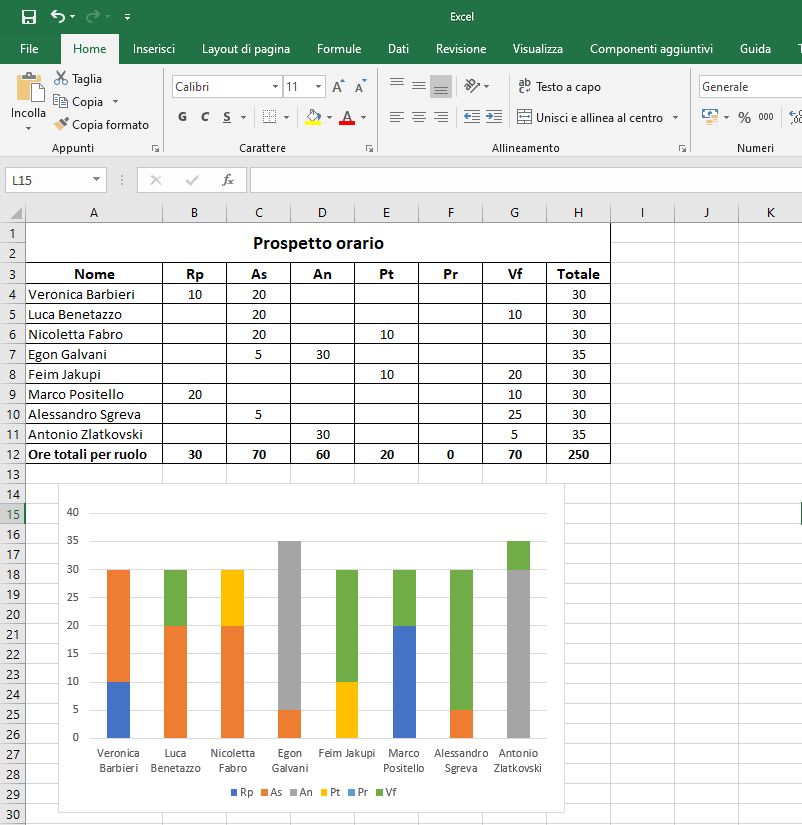
\includegraphics[scale=0.62]{./res/img/excel.png}
			\caption{Microsoft Excel}
		\end{figure}
		\pagebreak
	  \subsubsubsection{GanttProject}
	    Software per la gestione dei progetti basato su Java\ped{\textit{G}}. Utilizzato principalmente per la creazione di diagrammi di Gantt, ovvero strumenti in grado di rappresentare le tempistiche e le attività di un progetto, per tracciare quindi il suo avanzamento.
	    \begin{figure}[h!]
	    	\centering
	    	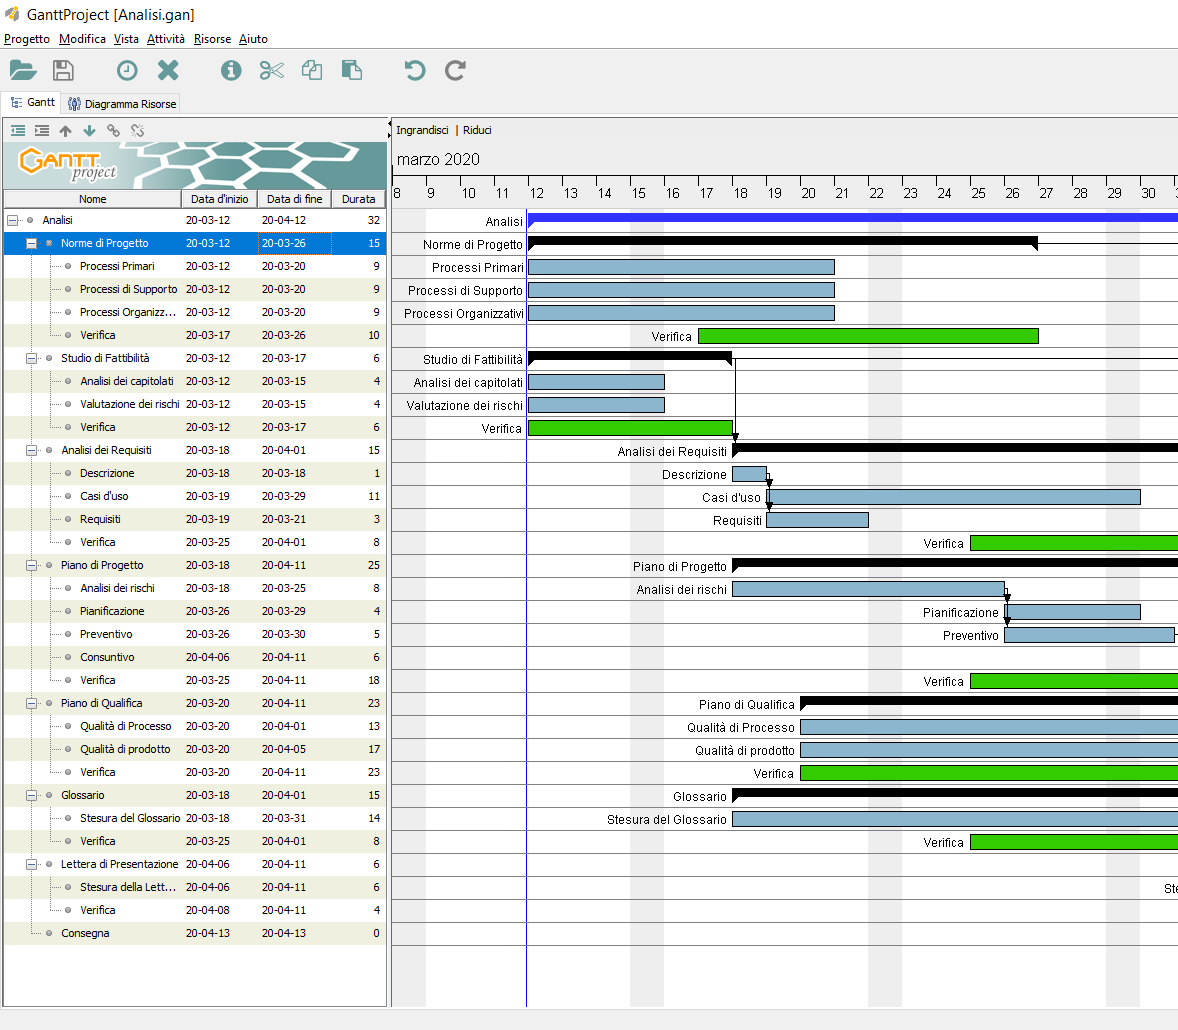
\includegraphics[scale=0.5]{./res/img/diagr_gantt.png}
	    	\caption{GanttProject}
	    \end{figure}
	    \pagebreak
		